\section{Indledning}
Der er til dette projekt ønsket et tracking system, et sådan system kan bruges til tracking af lydkilder, personer og/eller afstandsmåling, fælles for disse former for tracking er at de er styret af et pan-tilt system.

Dette projekt vil fokusere på at følge himmellegemer med en teleskop-platform. Dette bliver implementeret ved at give systemet angulære koordinater, enten udregnet via en computer som kan sende koordinaterne videre gennem UART, eller ved manuelt input fra et keyboard. Ved input fra computeren, vil der være mulighed for at lave en applikation, der automatisk følger et himmellegeme, ved at ændre koordinat inputtet hele tiden.
Systemet vil sende data tilbage til brugeren og vise dette på et LCD, her vil det være muligt at se hvilke grader systemet står på.

Pan-tilt systemet styres af en FPGA, som sender et PWM signal til en H-bro og videre til motoren som styrer hhv. pan og tilt.
FPGA’en skal modtage kommandoer fra en microprocessor via en SPI forbindelse.
Her har brugeren mulighed for at sende inputs, samt få feedback af systemparametre.


%\begin{figure}[h]
%\centering
%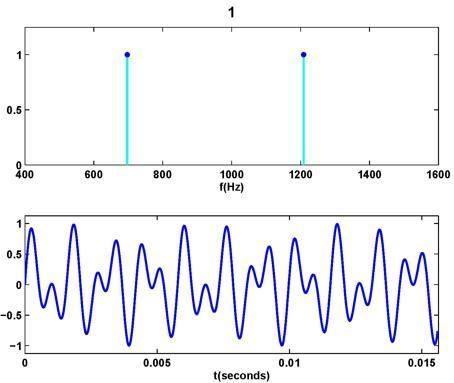
\includegraphics[scale=0.5]{Billeder/DTMF1.jpg}
%\caption{Relevant billede}
%\label{fig:DTMF1}
%\end{figure}